\section{Language Overview}
\label{sec:Overview}

The PORT language allows its users
to completely describe a mutator
that can
accept a given event stream if it contains a particular
activity sequence. But, it can also produce a modified
output event stream
for application testing.
As noted in Section 2, standard
deterministic automata or transducers can not accommodate these features.
Therefore, we instead compile a PORT program into
an  enhanced transducer that can operate over complex data structures.
The transducer consists of states, one of which is marked as the ``current state'', and
a series of rules that govern when the current state should change based on the event type
and the parameters of an input stream element.
Additionally, these rules describe what modifications should be made to the input stream.

The rules cited above consist of logical comparisons between an event's parameter values, the values stored in the transducer's registers, or the literals specified directly in a program's code.
Using event processing techniques, PORT maps activity onto a
stream of \emph{events}, which can be defined here as individual interactions between the program and its environment, e.g.,
a single library, system, or remote procedure call.
Each event consists of a unique identifier (e.g. the name of the function being called) and a list of parameter values (e.g. the argument and return values of the called function).
Parameter values are drawn from a set of basic data values, such as strings and numbers, as well as user-definable record types.

PORT allows the user to ignore parameter values that are irrelevant for the particular task at hand.  It also can create a single abstract event from several that are semantically related, but have different event identifiers. The transducer description can then refer to just these abstract events rather than individually specify each event it contains.

A PORT transducer processes an input event stream as follows (illustrated in Figure~\ref{fig:Processing}).
Each item in an input
sequence is examined and the transducer's internal state is updated accordingly.
 Output is then produced based on the rules described in the transducer's program.
 In this way, 
 the transducer itself can be thought of as a sequence of \emph{actions}
 that may or may not be executed based on the values in the input stream. 
 The state of the transducer keeps track of the next action to be executed, as well as a valuation of a 
 finite number of \emph{registers} that hold data values.
 Whether or not an action is executed depends on a combination of the transducer state
 and the values of the current event.
 Therefore, executing an action consists of reading the next
event from the input stream, which may update some of the registers, and then writing the next event in the output stream.
%The parameter values in the output event may be computed from the (updated) registers.

\begin{figure}[t]
  \centering
  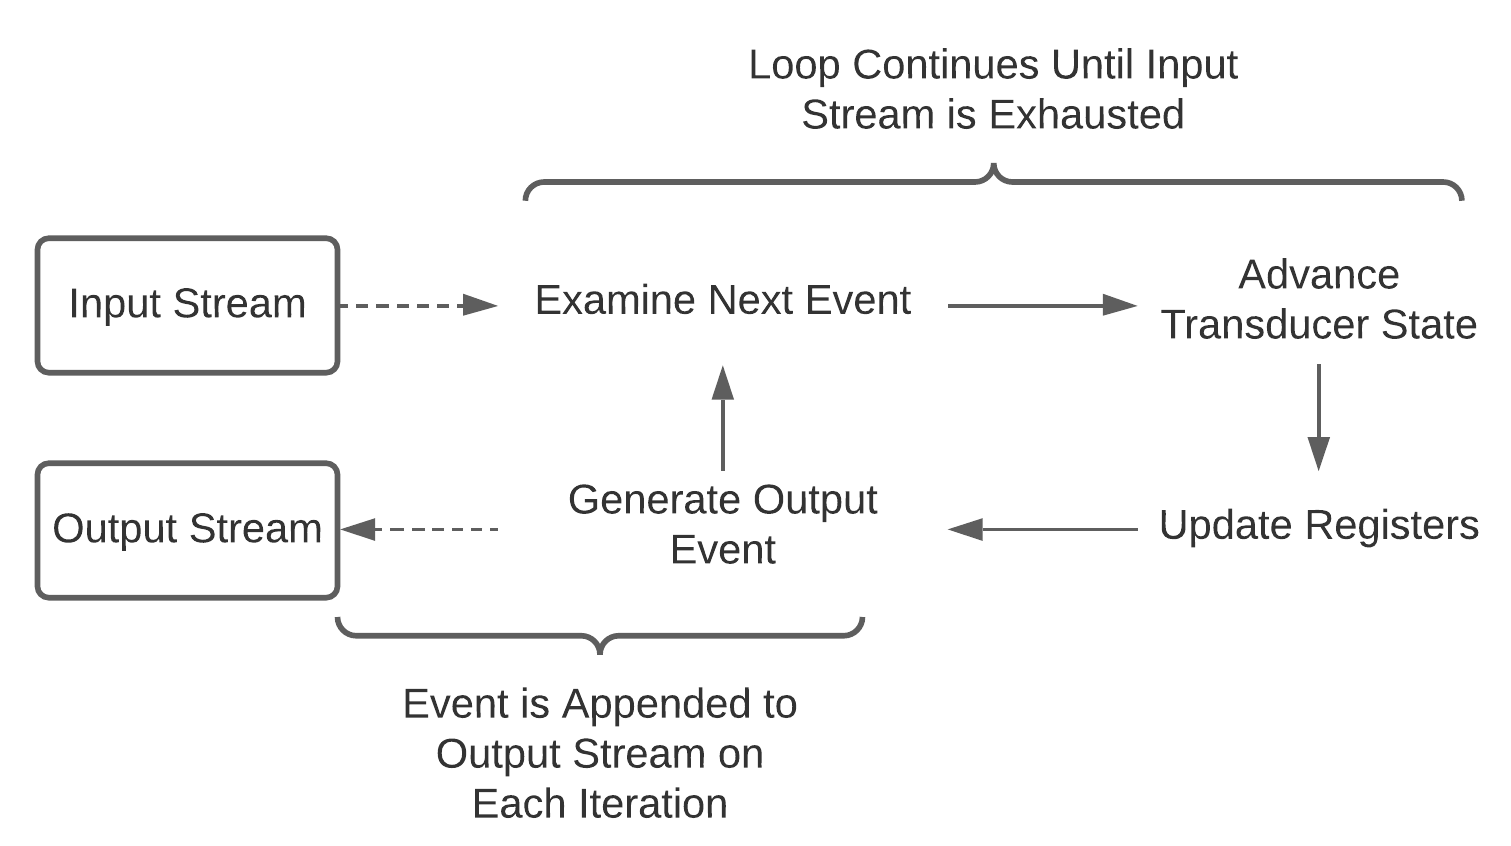
\includegraphics[scale=.6]{images/processing}
  \caption{A transducer individually processes each item in an input
  sequence, updating its internal state and producing output according
  to the rules described in its program.}
  \label{fig:Processing}
\end{figure}

%\iffalse
%Each action either processes a single event from the input stream, possibly additionally updating some registers of the transducer.
%
%This arrangement allows a user to find
%a specific category of events
%in a stream
%by matching a set of desired properties.
%To do so, the system specifies
%an identifier and a set of parameter value
%constraints.  For example, an unsuccessful {\tt close()} call could be
%found by looking for events with the identifier {\tt close} and a return
%value of -1.  This pairing of an identifier and a set of parameter
%constraints, referred to as an \emph{event pattern}, forms the primary mechanism in PORT for
%selecting specific events out of an activity stream.
%
%Implementing
%a program written in PORT 
%to identify a pattern of activity works as follows.
%As illustrated in Figure~\ref{fig:Processing}, a pattern is encoded as a list of datawords, and compared against
%events from the
%input event stream until the first dataword
%finds a ``match'' (matching is discussed further in
%Section~\ref{sub:PreambleAndBody}).  The event stream is next matched
%against the
%second dataword
%and so on until all datawords have been matched or the event stream is
%exhausted.
%
%
%%% talk about output.
%%Output is achieved through one further addition -- an output clause.  This
%%clause may be applied to any of the datawords in the list and describes
%%what output should be produced when the dataword it is associated with
%%matches an event.
%%
%%Datawords without an output clause are simply output without modification.
%%
%%In the following sections we discuss how these elements may be written as a
%%PORT program and transformed into a working mutator.
%
%
%\subsection{Preamble and Body}
%\label{sub:PreambleAndBody}
%
%\begin{figure}[h]
%\centering
%\begin{tabular}{c}
%\begin{lstlisting}
%########## Preamble ##########
%type statbuf {dev: String@0, stino: String@1};
%event fstat {fd: Number@0, st: statbuf@1};
%
%##########   Body   ##########
%finddev <- "st_dev=makedev(0, 4)";
%findino <- "st_ino=4026532069";
%out1 <- "foo";
%out2 <- "bar";
%fstat({st: {dev: ?finddev, stino: ?findino}});
%fstat({st: {dev: !finddev2, stino: !findino2}});
%fstat({st: {dev: ->out2, stino: ->out2}});
%\end{lstlisting}
%\end{tabular}
%\caption{An example PORT program with its preamble and body sections
%  labeled.}
%\label{lst:PreambleBody}
%\end{figure}
%
%
%
%A PORT program can be divided into two sections, the preamble and the body, as shown in
%Figure~\ref{lst:PreambleBody}. 
%The preamble defines the sorts of events
%expected
%to appear in an input event stream and the set of parameters
%under which future datawords will operate.  Specifying this information
%up-front configures a PORT mutator to
%automatically ignore extraneous information from the incoming stream.  This
%means that subsequent body statements only have to deal with events and
%parameters pertinent to the goal of the program.
%
%The body of a PORT program consists of a list of datawords that
%will configure the states and transitions
%of a mutator. 
%Each dataword (excluding usages of the NOT operator, discussed further
%in~\ref{subsub:NOT}) configures a single
%state and sets the rules that will govern how the mutator transitions into that state.
%Transitioning  into a new state is dependent on whether
%the current event``matches'' the requirements of the destination state.
%In PORT, a match requires satisfying three rules:
%
%\begin{itemize}
%\item{The event's identifier must match the destination state's identifier}
%\item{All parameters with the match operator applied must have a value equal to
%  the value currently stored in the associated register (discussed further
%    in Section~\ref{sub:DatawordOperators})}
%\item{All predicates must be satisfied by the parameter values in the
%  current event}
%\end{itemize}
%
%\fi


\subsection{Syntax and Semantics}
\label{sub:SyntaxAndSemantics}

Figure~\ref{lst:SyntaxGrammar} shows the grammar of PORT's core language.
A program is split into two parts: the \emph{preamble} consisting of type and event definitions, and the \emph{body} of the program which consists of a sequence of actions. 

\begin{figure}[t]
\centering
\scriptsize
\begin{minipage}[t]{.5\linewidth}
\begin{align*}
\mathit{program} ::= {} &  (\mathit{typedef} \mid \mathit{eventdef})^* \; \mathit{action}^*\\
\mathit{typedef} ::= {} & \mathtt{type}\; \mathit{id} \texttt{\{}\mathit{id} \texttt{:}\, t\, \texttt{@}\, n \; (\texttt{,} \mathit{id}\texttt{:} t\,\texttt{@}\,n)^*\texttt{\};}\\
\mathit{eventdef} ::= {} & \mathtt{event}\; \mathit{id} \; \mathit{variant} \; (\texttt{|}\; \mathit{variant})^*\texttt{;}\\
\mathit{variant} ::= {} & \texttt{\{}\mathit{id}\; \mathit{id}\texttt{:}\, t\,\texttt{@}\,n \; (\texttt{,} \mathit{id}\texttt{:}\, t\,\texttt{@}\,n)^*\texttt{\}}\\
%\mathit{body} ::= {} & \mathit{action}^*\\
%\mathit{action} ::= {} & \mathit{assignment} \mid \mathit{event}\\
%\mathit{assignment} ::= {} & \mathit{regid} \texttt{ <- } e\\
\mathit{action} ::= {} & \mathit{pattern} \texttt{ -> } \mathit{id}\,(e) \texttt{;} \mid \mathtt{not} \; \mathit{pattern} \texttt{;}\\
\mathit{pattern} ::= {} & \mathit{id}\,(p) \;\mathtt{with}\; b
\end{align*}
\end{minipage}%
\begin{minipage}[t]{.5\linewidth}
\begin{align*}
p \in \mathsf{pexp} ::= {} & \texttt{\{} \mathit{id}\texttt{:}\, p \; (\texttt{,} \mathit{id}\texttt{:}\, p)^*\texttt{\}} \mid \mathit{regid} \mid c \\
e \in \mathsf{vexp} ::= {} & \mathit{regid} \mid c \mid e \,\texttt{+}\, e \mid e \,\texttt{-}\, e \mid \dots\\
b \in \mathsf{bexp} ::= {} & \mathtt{true} \mid \mathtt{false} \mid e == e \mid \ldots \mid p \;\mathtt{and}\; p \mid \dots\\
t \in \mathsf{texp} ::= {} & \mathtt{String} \mid \mathtt{Number} \mid \mathit{id} \mid \dots
\end{align*}
\end{minipage}
\caption{Grammar of PORT's core language.}
\label{lst:SyntaxGrammar}
\end{figure}

\paragraph*{Preamble}

The abstract event consists of a name and a record of named fields that hold data values of interest. As an example, consider the event definition:
\begin{lstlisting}[numbers=none,xleftmargin=0em,gobble=2,columns=strict]
  event rd {read fdesc: Number@0} | {recv fdesc: Number@0};
\end{lstlisting}
This definition maps the concrete events named \lstinline+read+ and \lstinline+recv+ to the abstract event \lstinline+rd+. The parameter values of the concrete events are abstracted to a record consisting of a single field \lstinline+fdesc+ that holds a value of type \lstinline+Number+. The notation \lstinline+fdesc: Number@0+ in each variant indicates that the value of \lstinline+fdesc+ is the 0th parameter of the corresponding concrete event. Note that all variants must map their parameters to the same record type.

If an event definition defines an abstract event in terms of a single variant for which the concrete event name coincides with the name of the abstract event, then the former can be omitted in the variant.

Event definitions have three distinct functions. First, they allow a PORT program to ignore
irrelevant parameter values in concrete events. Second, they can map semantically-related concrete events to the same abstract event, and lastly it permits any modifications of record fields to be mapped back to corresponding modifications of the underlying concrete events.
%These operations can be accomplished even if the values tracked by the
%abstract event occur at different positions in the parameter lists of the concrete events.

The abstraction mechanism used for the parameter lists of concrete events can also be applied to the values themselves. For instance, the 1st parameter of an \lstinline+fstat+ system call is a status buffer that consists of a list of values. \emph{Type definitions} can be used to abstract such compound values into records. The following PORT code defines an abstract \lstinline+fstat+ event that tracks only the device identifier, inode number, and mode of the status buffer:
\begin{lstlisting}[numbers=none,xleftmargin=0em,gobble=2]
  type SB {dev: String@0, ino: String@1, mode: String@2};
  event fstat {fdesc: Number@0, sbuf: SB@1};
\end{lstlisting}

%\iffalse
%Each statement specifies an event ``variety'' and a list of
%parameters that should be accessible in later dataword statements.
%An event's variety will correspond
%with the system call name, RPC call name, or, in the case of other activity
%representations, a unique identifier that allows events of the same
%variety to be picked out of a stream.
%
%A variant definition allows several event definitions to be combined under
%a single identifier.  This identifier may then be used in a dataword
%statement to match any of the collected events.
%
%  This feature arose as a
%result of situations where one of several system calls could be used to
%perform the same operation (e.g. {\tt read()} and {\tt recv()}).  The
%concrete syntax necessary to achieve this pairing is shown in the example
%above where the variant ``bothread'' is defined such that it will match
%either a {\tt read()} or {\tt recv()} system call.
%\fi



\paragraph*{Body}
The actions in the body of a PORT program describe how the input event stream is transformed to the output event stream. An individual input event is matched and transformed by an action of the form
\[\mathit{id}_1(p) \;\mathtt{with}\; b \texttt{ -> } \mathit{id}_2\,(e)\texttt{;}\]
This action matches the next (abstract) input event against the \emph{pattern} $\mathit{id}_1(p)$ subject to the constraint $b$. The action is triggered if the name of the matched event is $\mathit{id}_1$ and its record satisfies the constraints imposed by $p$ and $b$. The semantics of pattern matching is similar to the way  expressions are pattern matched in functional programming languages. In particular, a variable occurring in a pattern refers to a register of the transducer. If the pattern matches the event, then the register is assigned to the corresponding value. For example, consider the pattern:
\begin{lstlisting}[numbers=none,xleftmargin=0em,gobble=2]
  fstat({fdesc: fd2, sbuf: {dev:rdev, stino: rino2}})
\end{lstlisting}
When matched against the event%\\
%\begin{adjustbox}{max width=\textwidth}
\begin{lstlisting}[numbers=none,xleftmargin=0em,gobble=2,basicstyle=\ttfamily\footnotesize]
  fstat({fdesc: 4, sbuf: {dev:"st_dev=makedev(0, 4)", ino: 42, mode="S_IFCHR|0666"}})
\end{lstlisting}
%\end{adjustbox}\\
the match would succeed and assign the value \lstinline+4+ to register \lstinline+fd2+, \lstinline+"st_dev=makedev(0, 4)"+ to register \lstinline+rdev+, and \lstinline+"S_IFCHR|0666"+ to register \lstinline+rino2+.

The Boolean expression $b$ is evaluated after the initial match of $\mathit{id}_1(p)$ succeeds. If $b$ evaluates to \lstinline+true+ then the action takes effect. Otherwise, the match fails and the registers are reset to their original values before $\mathit{id}_1(p)$ was matched.

When an action takes effect, the matched input event is consumed and an output event is appended to the output stream. This output event is described by $\mathit{id}_2\,(e)$ in the \emph{output clause} of the action. If $\mathit{id}_2=\mathit{id}_1$, then $e$ can be a \emph{partial} record expression, describing only those parts of the input record that should be modified by the action. Record fields that are not specified by $e$ are copied from the input event to the output event. If the record types of the input and output events differ, $e$ must describe the output record completely.

For example, consider the action:
\begin{lstlisting}[numbers=none,xleftmargin=0em,gobble=2]
  fstat({fdesc: rfd2, sbuf: {dev:rdev, ino: rino2}})
    with rfd2 == rfd and rdev == "st_dev=makedev(0, 4)" -> fstat({sbuf:{ino: rino}});
    \end{lstlisting}
This action matches the \lstinline+fstat+ event given above, assuming the register \lstinline+rfd+ has value \lstinline+4+ before the match. Moreover, if the register \lstinline+rino+ has value \lstinline+43+ before the action is executed, then the action produces the output event:
\begin{lstlisting}[numbers=none,xleftmargin=0em,gobble=2]
  fstat({fdesc: 4, sbuf: {dev:"st_dev=makedev(0, 4)", ino: 43, mode="S_IFCHR|0666"}})
  \end{lstlisting}

For convenience, we have included a syntactic short-hand that allows one to more compactly express common kinds of patterns. First, one often needs to express that the value of a matched record field is equal to the current value of a register. In the action above, the field \lstinline+fdesc+ of the matched \lstinline+fstat+ event must be equal to \lstinline+rfd+ for the match to succeed. This constraint can be expressed more succinctly by replacing \lstinline+rfd2+ with \lstinline+?rfd+ in the pattern of the action. Doing so ensures that the matched value is equal to \lstinline+rfd+ without changing the value of \lstinline+rfd+. The equality \lstinline+rsd2 == rsd+ can then be omitted from the \lstinline+with+ clause.

Next, the \lstinline+with+ clause can also be omitted altogether from an action, in which case $b$ defaults to \lstinline+true+. Likewise, the output clause can be omitted and the matched input event can simply be copied to the output stream. Finally, an action is replacing only the value of a field, and the action is not dependent on the old value, then the modified field value can be specified directly in the pattern using the notation \lstinline+->$e$+. Here, the expression $e$ determines the new value to be stored in the field.

Using this syntactic short-hand, the action given above can be expressed more compactly as:
\begin{lstlisting}[numbers=none,xleftmargin=0em,gobble=2]
  fstat({fdesc: ?rfd, sbuf: {dev:"st_dev=makedev(0, 4)", ino: -> rino}});
\end{lstlisting}


\paragraph*{Implicit repetition and negated patterns}
%In our design of PORT we have decided against the inclusion of the repetition and choice constructs supported by general-purpose stream processing languages. This design decision greatly simplifies the transducer construction as we do not have to deal with elimination of epsilon transitions expressing nondeterministic choice. 

PORT simplifies the handling of an unbounded input stream by using implicit repetition semantics.
Any event in the input stream not matched by the current action is simply copied to the output stream. The transducer moves on by attempting to match the next input event against the current action.

Sometimes, it is necessary to constrain this implicit repetition mechanism by disallowing the appearance of certain events in the input stream before an event  matched by the current action is encountered.  This can be done by \emph{negated patterns}, which take the form \lstinline+not id$(p)$ with $b$+. If an event that matches the pattern \lstinline+id$(p)$ with $b$+ is encountered before the next positive action in the program takes effect, then the transducer aborts. For instance, the PORT program in Fig.~\ref{fig:CompareListing} uses a negated pattern to ensure that no \lstinline+read+ system call is executed on the opened file with file descriptor \lstinline+fd+ before the file is closed.

\paragraph{Explicit repetition}
PORT also supports matching clearly defined sequences of events.  This functionality is useful when a desired pattern
contains some unknown number of repetitions of one or more events.
This functionality behaves similarly to a Kleene star as provided by many regular expressions engines.
That is, the generated transducer accepts zero or more repetitions of the specified sequence of events.
Output is only produced if a complete repetition of sequence is encountered.
All previously discussed functionality and behavior holds true for the sequence being repeated.

%\iffalse
%This production triggers the creation of a mutator with only a starting
%state.  This state is accepting in two situations:
%\begin{itemize}
%  \item{When no other states are added to the automaton by subsequent
%    statements}
%  \item{When the only other states added to the automaton are NOT states
%    which reject sequences they match}
%\end{itemize}
%In all other cases this is a rejecting state that produces no output.
%
%
%\begin{quote}
%\centering
%\textbf{assignment: x <- e}
%\end{quote}
%
%Assignment statements store the value of an expression, e, into a named
%register on the mutator being described.
%If the register does not exist,
%it is created;
%otherwise its stored value is overwritten.
%Registers may contain Number or String values.  Register contents
%may be used in subsequent statements to specify parameter values that must
%be present in order for an event to match, or as values to be output.
%
%
%
%\begin{quote}
%\centering
%\textbf{dataword: id paramexp predexp outputexp}
%\end{quote}
%
%
%Dataword statements are responsible for adding new states to the
%mutator.  This means they must specify any register operations,
%transition conditions, and output associated with these new states.  To
%tackle this complexity we will address each part of this production
%individually.
%
%\textit{id paramexp}
%
%The parameter expression offers an opportunity to examine and store
%parameter values from the current event.  PORT supports two operators
%that may be applied to parameter expression members.  The match operator
%(!) allows for the rejection of otherwise matching events
%by enforcing a required value on a
%chosen parameter while the store operator (?) copies a value from the
%current event and stores it in the specified register.
%
%
%\textit{predexp}
%
%Predicate expressions are used to place additional restrictions that must
%be met if the mutator is to advance into the newly created state.  These
%restrictions compare values from the current event to either register
%values or literal values.
%
%\textit{outputexp}
%
%An output clause controls the output that will be produced when its
%associated state is entered.  The nature of this output is controlled by a
%parameter expression that specifies which parameters of the current event
%should be replaced with a value from a register.  If a parameter is not
%included in the parameter expression, its original value is used.
%Similarly,
%if an output clause is omitted, the output will be the
%original, unmodified event.
%
%\subsection{Dataword Operators}
%\label{sub:DatawordOperators}
%
%PORT supports two operators that may be applied to a dataword's
%parameters: Match and Store.  These operators are central components in
%the description of a mutator.  Each operator is associated with a dataword
%parameter and a register or literal value.
%
%\subsubsection{Store Operator (!)}
%
%The store operator, ``\textit{!}'', adds a requirement that the
%mutator should extract a parameter value from the current event and store
%it in the specified register.  These values may then be modified by
%register expressions, combined with the match operator to add more
%entry requirements to a state, or used in output expressions.
%
%\subsubsection{Match Operator (?)}
%
%The match operator, ``\textit{?}'',
%allows PORT's user
%to provide additional conditions
%that an event's parameter values must meet
%in order to match a dataword.
%Specifically,
%the operator requires
%that its parameter value equal the
%register value
%or literal value
%to which it is applied.
%This functionality is
%useful when a value is stored upon the occurrence of one event
%and then used to identify an associated event expected to appear later.
%A common example of this pattern is storing the file descriptor
%returned by an {\tt open()} or {\tt socket()} call into a register
%and using it to find related {\tt read()} further along in a system call
%trace.
%
%\subsubsection{The NOT keyword}
%\label{subsub:NOT}
%
%The NOT keyword is used to reject a sequence if the event being
%described is encountered.  This is done by creating a ``trap''
%rejecting state.  Such a state follows the same entry rules
%as a normal state but has no outgoing transitions.  This guarantees that a
%recording containing matching events will be rejected.
%We found this capability useful for writing programs that could identify
%situations where an application incorrectly performs one or more steps of a
%complex operation.
%
%
%
%\fi
%
%%%%% We need to talk about how we are different from other
%%%%% languages that are regular-expression like here
%%\subsection{Inspiration from Regular Expressions}
%
%%%% Local Variables:
%%%% mode: latex
%%%% TeX-master: "paper"
%%%% End:
%
